% CVPR 2023 Paper Template
% based on the CVPR template provided by Ming-Ming Cheng (https://github.com/MCG-NKU/CVPR_Template)
% modified and extended by Stefan Roth (stefan.roth@NOSPAMtu-darmstadt.de)

\documentclass[10pt,twocolumn,letterpaper]{article}

%%%%%%%%% PAPER TYPE  - PLEASE UPDATE FOR FINAL VERSION
% \usepackage[review]{cvpr}      % To produce the REVIEW version
\usepackage{cvpr}              % To produce the CAMERA-READY version
%\usepackage[pagenumbers]{cvpr} % To force page numbers, e.g. for an arXiv version

% Include other packages here, before hyperref.
\usepackage{graphicx}
\usepackage{amsmath}
\usepackage{amssymb}
\usepackage{booktabs}


% It is strongly recommended to use hyperref, especially for the review version.
% hyperref with option pagebackref eases the reviewers' job.
% Please disable hyperref *only* if you encounter grave issues, e.g. with the
% file validation for the camera-ready version.
%
% If you comment hyperref and then uncomment it, you should delete
% ReviewTempalte.aux before re-running LaTeX.
% (Or just hit 'q' on the first LaTeX run, let it finish, and you
%  should be clear).
\usepackage[pagebackref,breaklinks,colorlinks]{hyperref}


% Support for easy cross-referencing
\usepackage[capitalize]{cleveref}
\crefname{section}{Sec.}{Secs.}
\Crefname{section}{Section}{Sections}
\Crefname{table}{Table}{Tables}
\crefname{table}{Tab.}{Tabs.}


%%%%%%%%% PAPER ID  - PLEASE UPDATE
\def\cvprPaperID{*****} % *** Enter the CVPR Paper ID here
\def\confName{CVPR}
\def\confYear{2023}


\begin{document}

%%%%%%%%% TITLE - PLEASE UPDATE
\title{Power Grid Vulnerability Analysis, A Complex Network Story}

\author{Renan Monteiro Barbosa\\
University of West Florida\\
11000 University Parkway, Pensacola, FL 32514, United States of America \\
{\tt\small rmb54@students.uwf.edu}
% For a paper whose authors are all at the same institution,
% omit the following lines up until the closing ``}''.
% Additional authors and addresses can be added with ``\and'',
% just like the second author.
% To save space, use either the email address or home page, not both
\and
Bala Raju Pidatala\\
University of West Florida\\
11000 University Parkway\\
{\tt\small bp94@students.uwf.edu}
\and
Chantal Ojurongbe\\
University of West Florida\\
11000 University Parkway\\
{\tt\small czo1@students.uwf.edu}
}
\maketitle

%%%%%%%%% ABSTRACT
\begin{abstract}
    This paper examines the structural vulnerability of power grid infrastructure through the lens of complex network theory. By modeling the grid as a graph, the study employs centrality metrics — specifically Degree and Betweenness Centrality — to identify critical components. Vulnerability is assessed by simulating network disruptions, comparing the impact of random node failures (RND) against targeted attack strategies: Initial Degree (ID), Initial Betweenness (IB), Recalculated Degree (RD), and Recalculated Betweenness (RB). Findings indicate that Betweenness Centrality-based attacks, especially the Recalculated Betweenness (RB) strategy, are markedly more effective at fragmenting the network than degree-based or random removal strategies. This underscores the critical importance of nodes serving as bridges between network regions, which Betweenness Centrality effectively identifies. The research concludes that power grid topology is highly susceptible to targeted attacks on these bridging elements, suggesting that resilience efforts should prioritize the protection of components crucial for maintaining network connectivity. The presented analysis relies significantly on visual interpretation due to technical limitations encountered during the study, which prevented the implementation of more advanced algorithms explored within TIGER.
\end{abstract}

%%%%%%%%% BODY TEXT

% ##############################################################################
% Introduction
% ##############################################################################

\section{Introduction}
\label{sec:intro}

The potential vulnerabilities of the American power grid for a prolonged collapse have been the focus of several documentaries, movies, Congressional hearings and commissions and they live in the imagination of the public. The electrical power grid vulnerabilities and eventual grid collapse due to geomagnetic storms, electromagnetic pulse, cybersecurity, and cyberattacks as regards power plants and more seem to be more an imminent reality than a Fiction. So to understand more about the topic the intent of this report is to provide an objective summary of the current science and controversies on this issue.

%-------------------------------------------------------------------------
\subsection{The Criticality and Fragility of Power Grids}
% \textbf{The Criticality and Fragility of Power Grids}

Modern civilization is intrinsically linked to and deeply reliant upon the continuous and reliable supply of electrical power. Power grids function as the operational backbone for nearly all facets of contemporary life, underpinning economic stability, ensuring national security, supporting public health systems, and enabling essential daily activities \cite{number1}. 
% (Add a citation number 1). 
These vast networks are not merely independent entities; they are foundational critical infrastructures upon which other vital systems, such as telecommunications, transportation, water supply, and financial services, depend. \cite{ani2019review} 
% (add a citation number 5) 
The interconnected nature of modern infrastructure means that disruptions within the power grid can cascade, causing widespread societal and economic paralysis.

Despite their criticality, power grids exhibit inherent fragility. Historical events serve as stark reminders of the potential consequences of grid failures. Large-scale blackouts, such as the 2021 Texas winter storm event \cite{number8} 
% (add a citation number 8) 
and the 2003 Northeast blackout \cite{number10}, 
% (add a citation number 10), 
have left millions without power, often under hazardous conditions. The economic repercussions are staggering, with individual events potentially costing billions of dollars in direct damages and lost productivity. \cite{number1} 
% (Add a citation number 1) 
Beyond economic costs, the human toll is significant. Power outages compromise public health by disabling heating and cooling systems during extreme temperatures, disrupting access to essential medical services, and causing spoilage of food and medication reliant on refrigeration. \cite{number1} 
% (Add a citation number 1) 
The 2021 Texas failure, for instance, not only caused widespread hardship but also brought the entire state grid perilously close—within minutes—to a complete collapse that could have taken weeks or months to restore, highlighting the potential for catastrophic, long-term disruptions. \cite{number8} 
% (Add a citation number 8) 
Similarly, the devastation following Hurricane Maria in Puerto Rico underscored the prolonged societal impact of grid failure, with extended outages contributing to significant excess mortality and immense economic loss. \cite{number10} 
% (Add a citation number 10)

%-------------------------------------------------------------------------
\subsection{Escalating Threats and Increasing Complexity}
% \textbf{Escalating Threats and Increasing Complexity}

The challenges facing power grid reliability are intensifying due to a confluence of escalating threats and growing system complexity. Climate change is driving an increase in the frequency and intensity of extreme weather events, which are a primary cause of power outages. \cite{number9} 
% (Add a citation number 9) 
Hurricanes, severe snow and ice storms, heatwaves, wildfires, and heavy rainfall events place immense physical stress on grid infrastructure, often exceeding the design limits of aging components. \cite{number1} 
% (Add a citation number 1) 
The 2021 Texas freeze \cite{number8} 
% (Add a citation number 8) 
and widespread summer heatwaves straining grids across the US \cite{number10} 
% (Add a citation number 10) 
exemplify this vulnerability. Aging transmission lines, transformers, and substations, many operating beyond their intended lifespans, are less resilient to these weather-related stresses. \cite{number1} 
% (Add a citation number 1)

% Citation number 2 raising errors \cite{number2}

Simultaneously, the cyber threat landscape is evolving rapidly. Power grids are increasingly reliant on digital control systems (e.g., SCADA) and interconnected technologies, creating new avenues for malicious actors. \cite{CraigFields} 
% (Add a citation number 2) 
Cyber-attacks targeting grid operations are growing in sophistication and frequency, with state-sponsored actors and criminal groups demonstrating the capability to disrupt or damage grid components. \cite{number9} 
% (Add a citation number 9) 
The integration of renewable energy sources, while beneficial for sustainability, introduces new potential vulnerabilities through distributed energy resources (DERs) like solar inverters and their associated communication networks, which may lack the robust security protocols of traditional, centralized power plants. \cite{number14} 
% (Add a citation number 14)

Physical threats also pose a significant and growing risk. Intentional attacks on substations and transmission infrastructure, including acts of sabotage, vandalism, and gunfire, have increased markedly in recent years. \cite{number14} 
% (Add a citation number 14) 
Copper theft from substations remains a persistent problem, causing damage and outages. \cite{number15} 
% (Add a citation number 15) 
Inadequate physical security measures and the vast, often remote, expanse of grid infrastructure make physical protection challenging. \cite{number15} 
% (Add a citation number 15)

These threats do not exist in isolation; they can interact and compound, creating scenarios far more damaging than standalone events. Extreme weather, for example, can physically stress the grid while simultaneously creating chaotic conditions that malicious actors might exploit for cyber-attacks, knowing the system is already vulnerable and response capabilities are strained. \cite{number20} 
% (Add a citation number 20) 
Studies simulating such compound cyber-physical threats have shown significantly amplified impacts, with unmet electricity demand potentially tripling compared to a cyber-attack alone.\cite{number20} 
% (Add a citation number 20) 
Furthermore, physical vulnerabilities, such as poorly maintained infrastructure or inadequate site security, can directly enable cyber intrusions by providing physical access to supposedly secure network components. \cite{number15} 
% (Add a citation number 15) 
This interplay necessitates a vulnerability assessment approach that considers the potential synergy between different threat vectors.

% Citation number 2 raising errors \cite{number2}

The inherent complexity of the grid itself magnifies these vulnerabilities. Power systems are vast, interconnected networks spanning large geographical areas, often operated by multiple entities. 
% ( Add a citation number 21, definition of power grid. Necessary ??? ) 
This interconnectedness, while providing operational flexibility, also creates pathways for failures to cascade rapidly across the system. \cite{kelic2017interdependencies} 
% (Add a citation number 6) 
The ongoing energy transition, involving the integration of diverse and often intermittent renewable energy sources and the deployment of smart grid technologies, further increases operational complexity. \cite{number14} 
% (Add a citation number 14) 
While modernization aims to enhance efficiency and control, it paradoxically introduces new types of interdependencies and potential failure points, particularly in the cyber domain. \cite{CraigFields} 
% (Add a citation number 2) 
This suggests a critical trade-off where technological advancements, if not implemented with integrated security and resilience considerations, can inadvertently expand the system's attack surface.

%------------------------------------------------------------------------
% ##############################################################################
% Methods
% ##############################################################################

\section{Methods}
\label{sec:methods}

% The outline for the Methods used in the research
% Briefly say you used Gephi and Python to study the network.
% Mention running:
% Centrality calculations (degree, betweenness, etc.)
% Community detection (modularity)
% Explain you removed:
% Top 10 important nodes (targeted attack)
% 10 random nodes (random failure)

In this study of graphs we refer as damaging the network as the removal of a node or edge in the graph. There are two primary ways a network can become damaged — (1) natural failure and (2) targeted attack. While random network failures regularly occur, they are typically less severe than targeted attacks. In contrast, targeted attacks carefully select nodes and edges in the network for removal in order to maximally disrupt network functionality. As such, we focus the majority of our attention to targeted attacks.

%------------------------------------------------------------------------
\subsection{Attack Strategies}

The attack strategies are assessesing the immediate impact of component removals on the network's structure and connectivity, without explicitly modeling power flow dynamics.The node removal strategies rely on node and edge centrality measures to identify candidates. Below, we highlight several attack strategies:

\begin{itemize}
    \item Random Node Removal (RND) - as the name suggests nodes or edges to be removed are picked at random.
    \item Initial degree removal (ID) - targets nodes with the highest degree. This has the effect of reducing the total number of edges in the network as fast as possible \cite{holme2002attack, beygelzimer2005improving}. Since this attack only considers its neighbors when making a decision, it is considered a local attack.
    \item Initial betweenness removal (IB) - targets nodes with high betweenness centrality. This has the effect of destroying as many paths as possible \cite{holme2002attack, beygelzimer2005improving}. Since path information is aggregated from across the network, this is considered a global attack strategy.
    \item Recalculated degree removal (RD) and Recalculated betweenness removal (RB) - follow the same process as ID and IB, respectively, with one additional step to recalculate the degree (or betweenness) distribution after a node is removed. This recalculation often results in a stronger attack.
\end{itemize}


%------------------------------------------------------------------------
% ##############################################################################
% Results
% ##############################################################################

\section{Results}
\label{sec:results}

% The outline for he results:
% Show what happened when you removed the top 10 nodes:
% Did the network split?
% Did the paths between nodes get longer?
% Show what happened when you removed random nodes:
% Did the network stay strong?
% Include a simple before/after comparison table if possible.

Attack success is measured based on how fractured the network becomes when removing nodes from the network. In the process of attacking the network we could identify three key observations — (1)random node removal (RND) is not an effective strategy at all on this network structure; (2) Recalculated Betweenness Removal (RB) is the most effective attack strategy; and (3) the remaining attacks are roughly equivalent, falling somewhere between RND and RB.

We could gain insight into why RB is the most effective of the attacks just by visual observations. If we look carefully, we observe that certain nodes (and edges) in the network act as key bridges between various network regions. As a result, attacks able to identify these bridges are highly effective in disrupting this network. In contrast, degree based attacks are less effective, likely due to balanced degree distribution and being locally limited. The analysis is similar for edge based attacks.

\begin{figure}[t]
    \centering
    % \fbox{\rule{0pt}{2in} \rule{0.9\linewidth}{0pt}}
    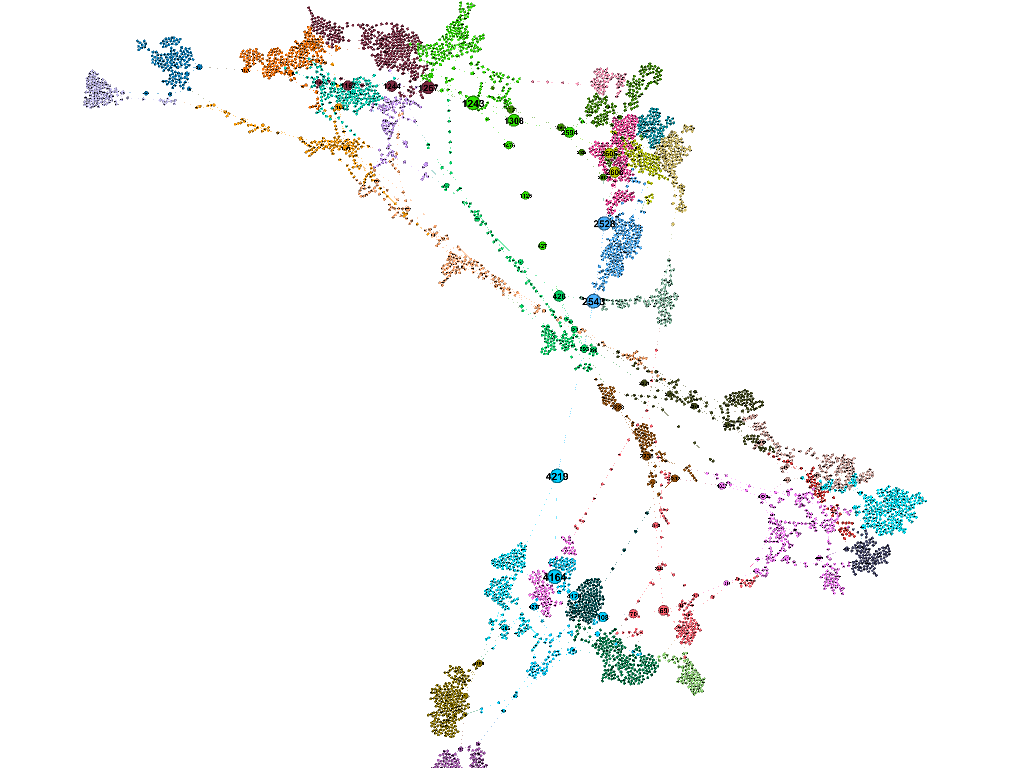
\includegraphics[width=0.8\linewidth]{images/PowerGrid_MC-BC2.png}
    \caption{After removing top 10 Betweenness Centrality.}
    \label{fig:onecol}
\end{figure}

\begin{figure}[t]
    \centering
    % \fbox{\rule{0pt}{2in} \rule{0.9\linewidth}{0pt}}
    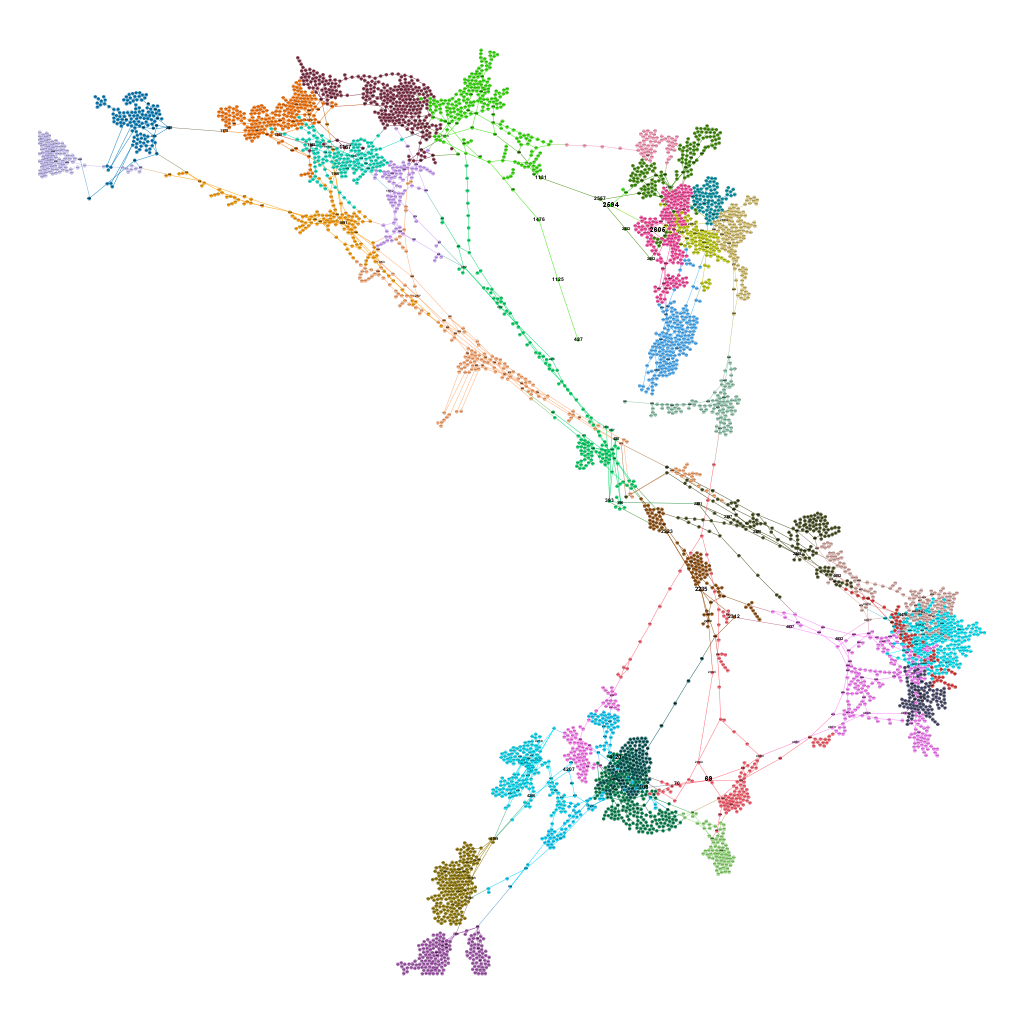
\includegraphics[width=0.8\linewidth]{images/PowerGrid_Targeted.png}
    \caption{Before removing top 10 Betweenness Centrality.}
    \label{fig:onecol}
\end{figure}

We can clearly see that Betweenness Centrality is a much more effective attack strategy, as well repeating this process we could observe that recalculating the Betweenness Centrality only compounded the effectiveness. Unfortunately due to python updates, deprecation in several packages and numerical instability with the Tensors. I could not implement a modern implementation of TIGER \cite{freitas2021evaluating}.


\begin{figure}[t]
    \centering
    % \fbox{\rule{0pt}{2in} \rule{0.9\linewidth}{0pt}}
    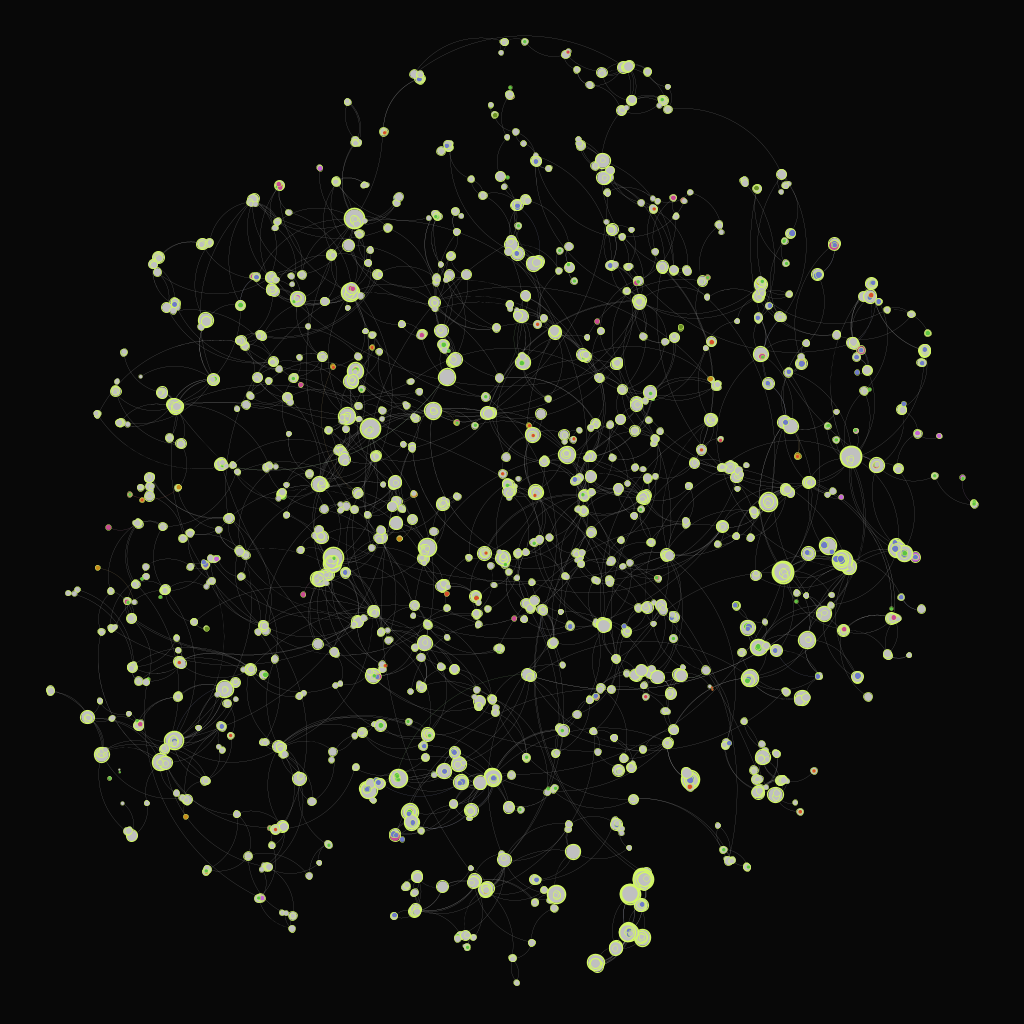
\includegraphics[width=0.8\linewidth]{images/Degree_power-targeted.png}
    \caption{After removing top 10 Degree Centrality.}
    \label{fig:onecol}
\end{figure}

\begin{figure}[t]
    \centering
    % \fbox{\rule{0pt}{2in} \rule{0.9\linewidth}{0pt}}
    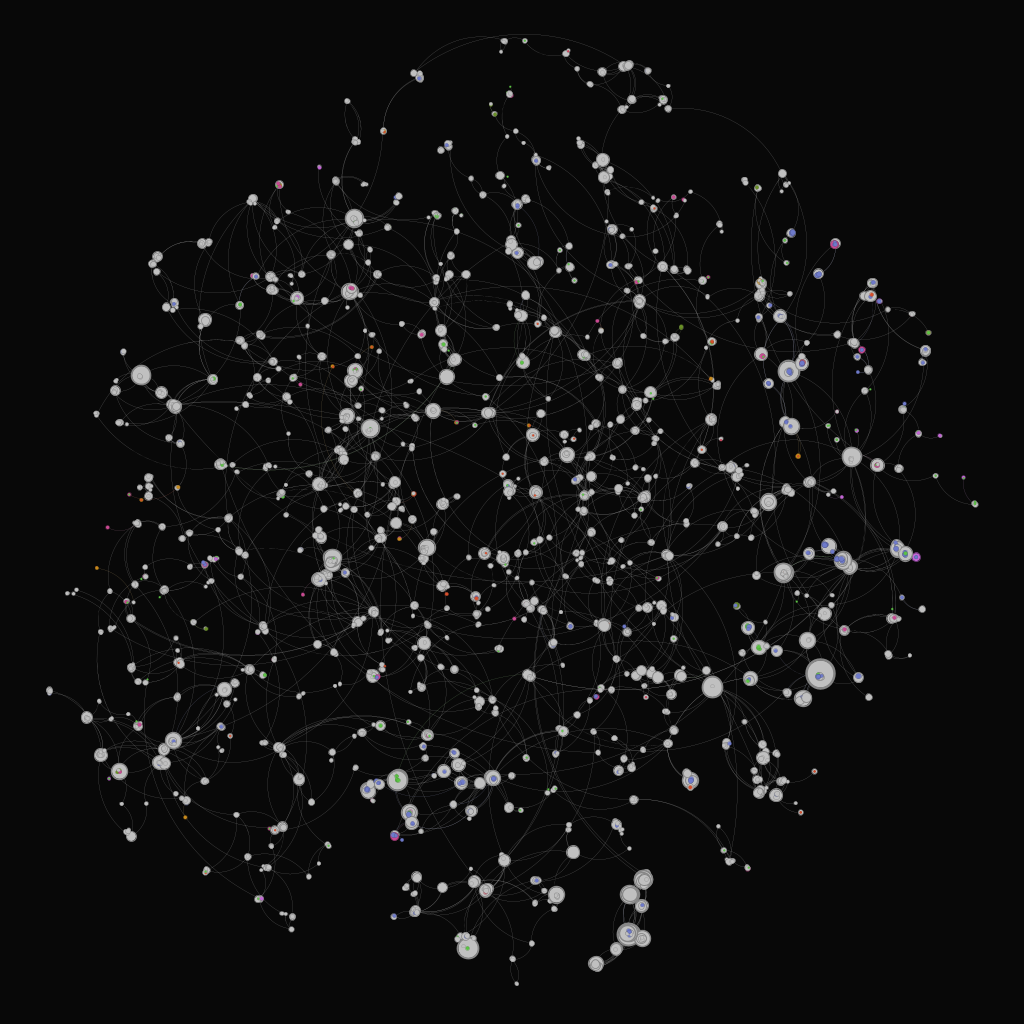
\includegraphics[width=0.8\linewidth]{images/Degree_power.png}
    \caption{Before removing top 10 Degree Centrality.}
    \label{fig:onecol}
\end{figure}

%------------------------------------------------------------------------
% ##############################################################################
% Conclusion
% ##############################################################################
\section{Conclusion}

This research outlines the systemic vulnerability of power grid infrastructures. Highlighting the value of modeling the grid as a complex network and employing siple but powerfull attack strategies based on well known network porperties.

We can conclude that we are more close to the total collapse of society than we could expect and through the use of simple tools we could avoid what could become an imminent catastrophe.

Also, would like to highlight that due to time contraints and technical difficulties the study was limited to visual observations and intuition rather than a robust implementation of algorithms.

% \cite{Authors14}

% \cite{Alpher02,Alpher03,Alpher05,Authors14b,Authors14}

%%%%%%%%% REFERENCES
{\small
\bibliographystyle{ieee_fullname}
\bibliography{egbib}
}

\end{document}
